\chapter{Vývojová dokumentácia}
\label{chap:vyvoj_dok}

Táto kapitola je zameraná pre programátorov, ktorých by bližšie zaujímali implementačné detaily a štruktúra nášho programu. Najprv si opíšeme ako skompilovať priložené zdrojové súbory práce a neskôr sa pozrieme na stavbu programu.

\section{Kompilácia}
V prílohe tejto práce sa nachádzajú zdrojové kódy nášho programu. Na ich úspešné skompilovanie budeme ale potrebovať splniť niekoľko požiadaviek:
\begin{itemize}
\item Podporovaná platforma na kompiláciu je momentálne iba Windows 10.
\item Ku kompilácii je potrebné Visual Studio 2019 s SDK verziou 10.0.19041.0
\item Qt verzie 5.15.0
\end{itemize}

\subsection{Inštalácia Qt}

Keďže ku kompilácii budeme potrebovať samotné Qt, ukážeme si jeho inštaláciu v nasledujúcich krokoch (v prípade, že náš počítač už obsahuje požadovanú verziu Qt, môžeme tieto kroky preskočiť a prejsť na integráciu VS s Qt~\ref{kap4:sec:VS2019_qt}). Tu je nutné spomenúť, že sa jedná o online inštaláciu a budeme potrebovať pripojenie k internetu:
\begin{itemize}
\item Po kliknutí  \href{https://www.qt.io/download}{\textbf{tu}} sa nám otvorí internetový prehliadač so stránkou na stiahnutie Qt, kde vyhľadáme možnosť \uv{Downloads for open source users} a klikneme na \uv{Go open source} (ukázané na obrázku~\ref{obr:kap4:qt_download}).

\begin{figure}[!htb]
	\centering
	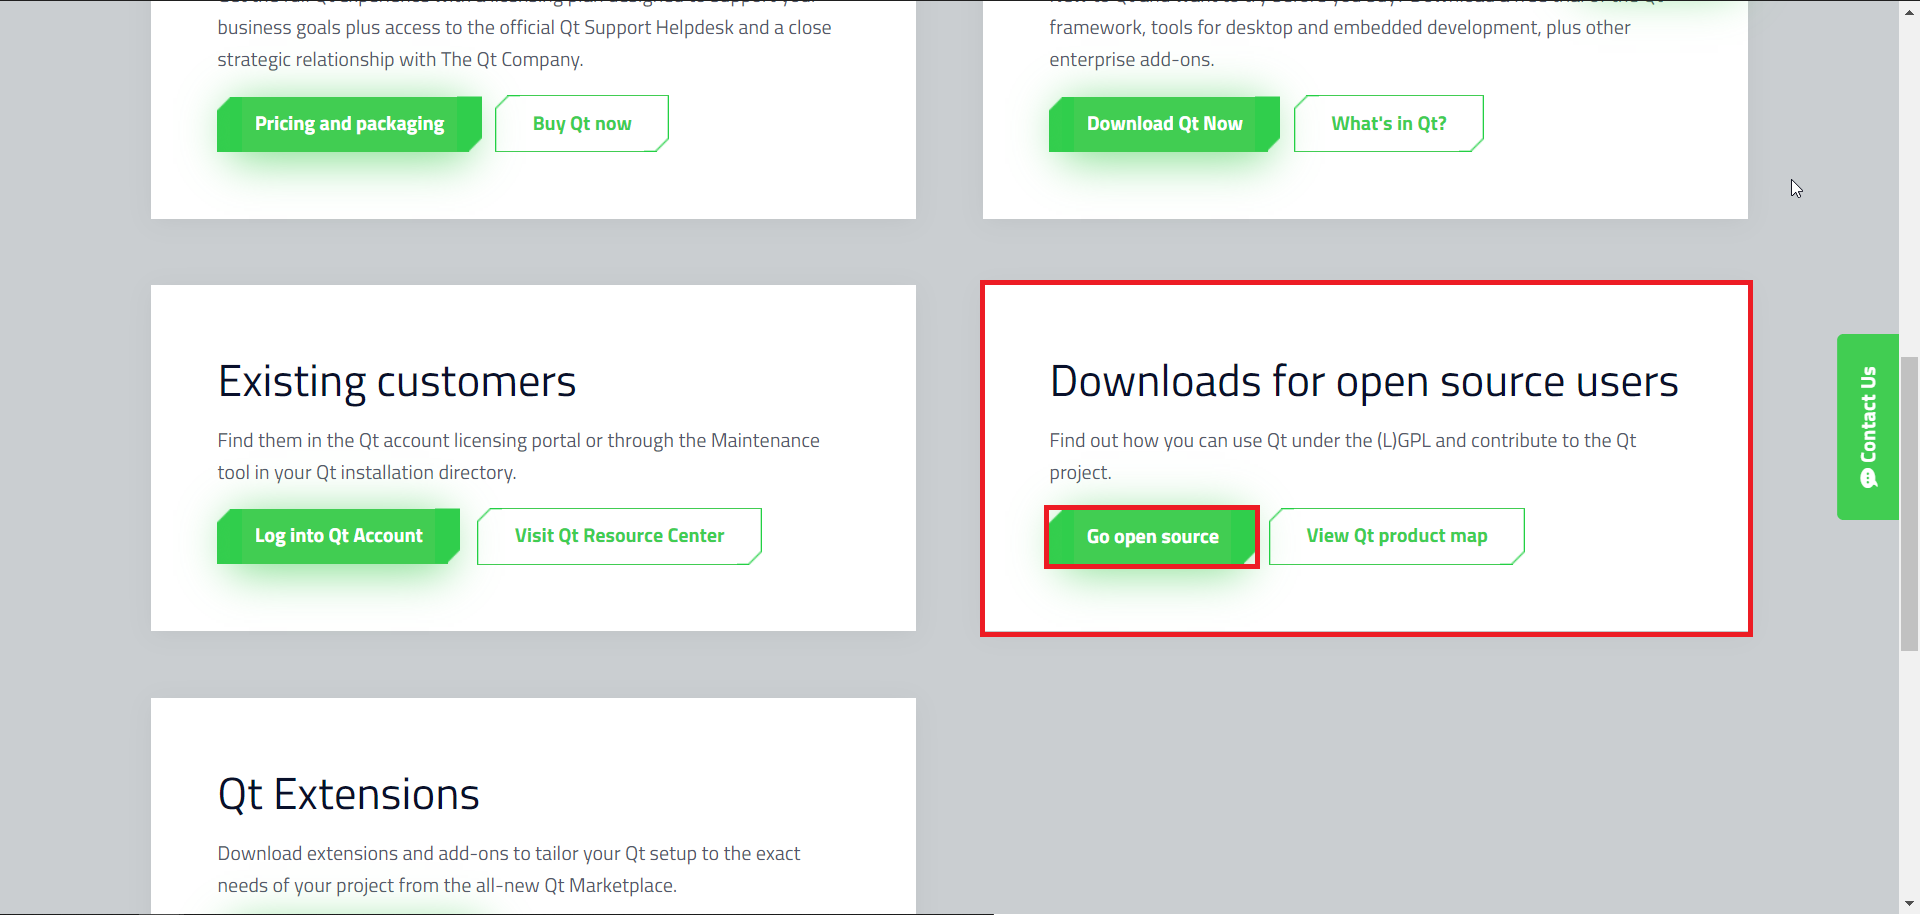
\includegraphics[width=12cm]{img/kap04_qt_download}
	\caption{Stránka Qt download.}
	\label{obr:kap4:qt_download}
\end{figure}

\item Na aktuálnej stránke nascrollujeme úplne dole, kde klikneme na zelené tlačidlo s nápisom \uv{Download the Qt Online Installer} (obrázok~\ref{obr:kap4:qt_online}).

\begin{figure}[!htb]
	\centering
	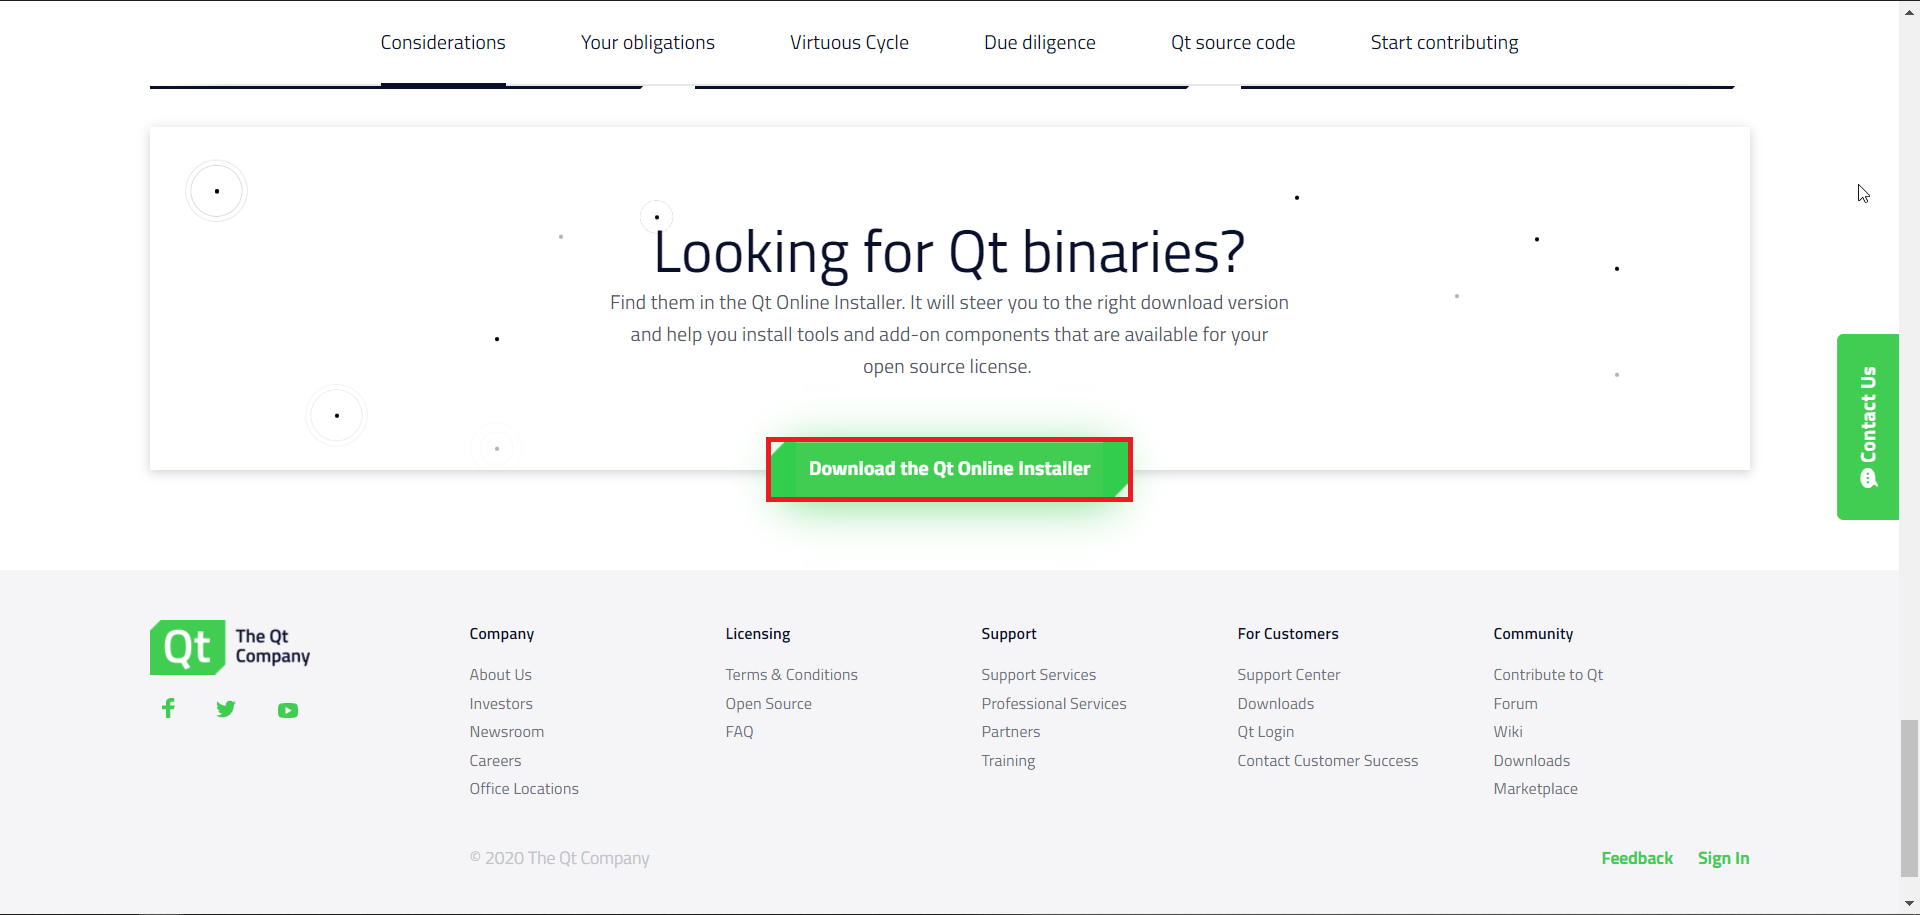
\includegraphics[width=12cm]{img/kap04_qt_online}
	\caption{Stránka Qt -- odkaz na stiahnutie \uv{Qt Online Installer}.}
	\label{obr:kap4:qt_online}
\end{figure}

\item Na aktuálnej stránke klikneme na \uv{Download}, čím sa nám stiahne \uv{Qt Online Installer}. Ten následne spustíme. Ukážku vidíme na obrázku~\ref{obr:kap4:qt_online_down}.

\begin{figure}[!htb]
	\centering
	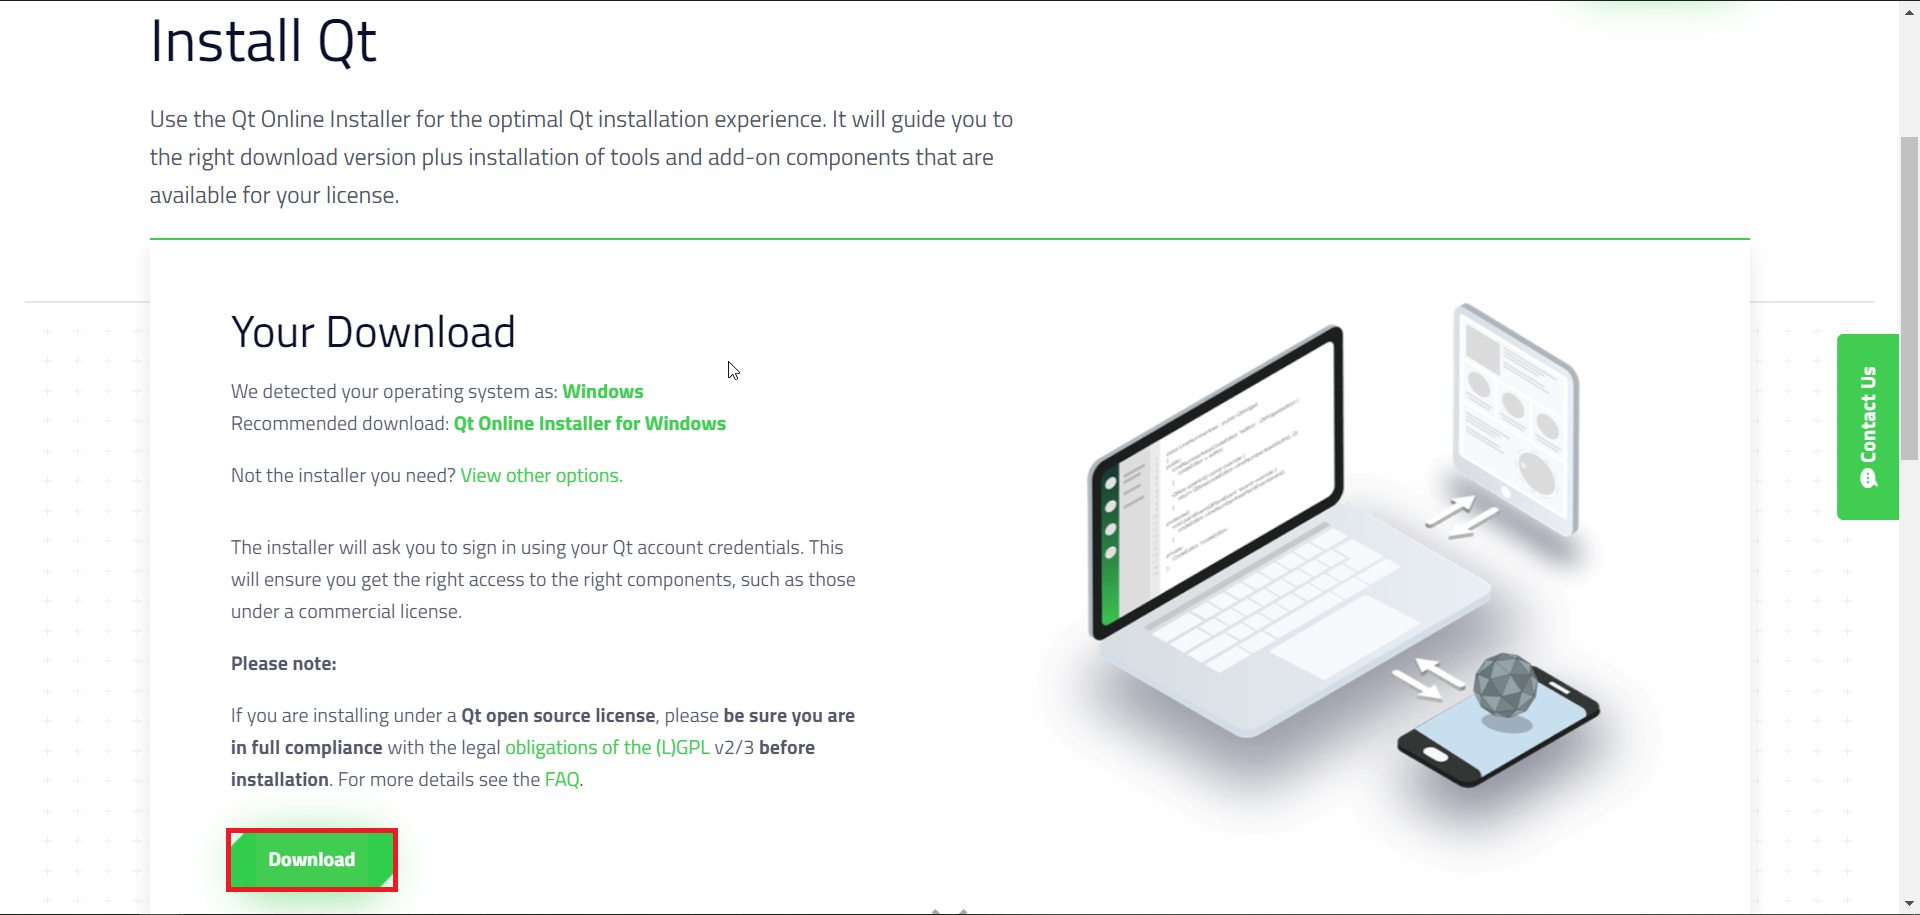
\includegraphics[width=12cm]{img/kap04_qt_online_down}
	\caption{Stránka Qt stiahnutie uv{Qt Online Installeru}.}
	\label{obr:kap4:qt_online_down}
\end{figure}

\newpage
\newpage

\item Ako prvé nás privíta obrazovka, ktorá od nás vyžaduje prihlásenie sa do nášho Qt účtu. Toto je bohužiaľ nutnosť a nie je možné bez toho pokračovať. V prípade, že nemáme žiadny vytvorený Qt účet, môžeme si ho vytvroiť priamo počas inštalácie a celé to nezaberie viac ako dve minúty. Potom klikneme na tlačidlo \uv{Next} (obrázok~\ref{obr:kap4:inst_welcome}).

\begin{figure}[!htb]
	\centering
	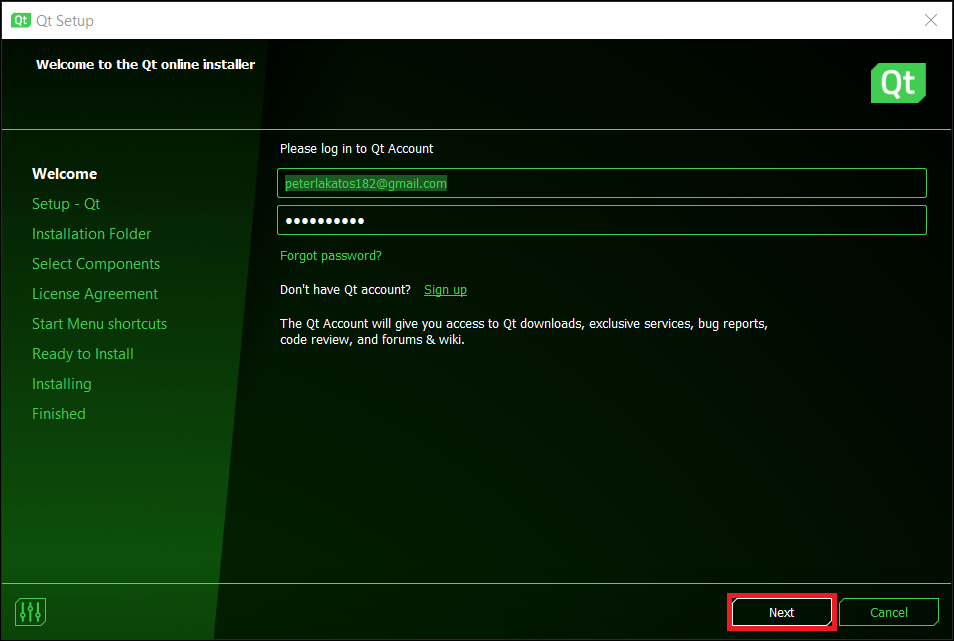
\includegraphics[width=12cm]{img/kap04_inst_welcome}
	\caption{\uv{Welcome} časť Qt Setupu}
	\label{obr:kap4:inst_welcome}
\end{figure}


\item Teraz zaškrtneme, že sme si prečítali a súhlasíme s povinnosťami používania \uv{Open Source Qt} a klikneme na tlačidlo \uv{Next} (obrázok~\ref{obr:kap4:inst_oblg}).

\begin{figure}[!htb]
	\centering
	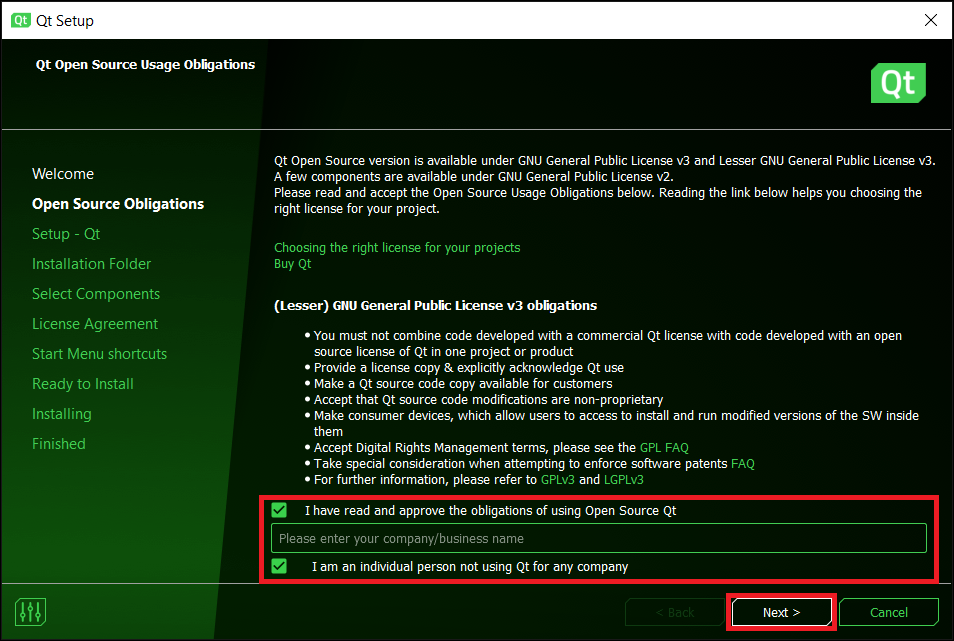
\includegraphics[width=12cm]{img/kap04_inst_oblg}
	\caption{\uv{Open Source Obligations} časť Qt Setupu}
	\label{obr:kap4:inst_oblg}
\end{figure}

\item Momentálne len klikneme na tlačidlo \uv{Next} a počkáme kým sa nám stiahnu dáta z repozitára (obrázok~\ref{obr:kap4:inst_set}).

\begin{figure}[!htb]
	\centering
	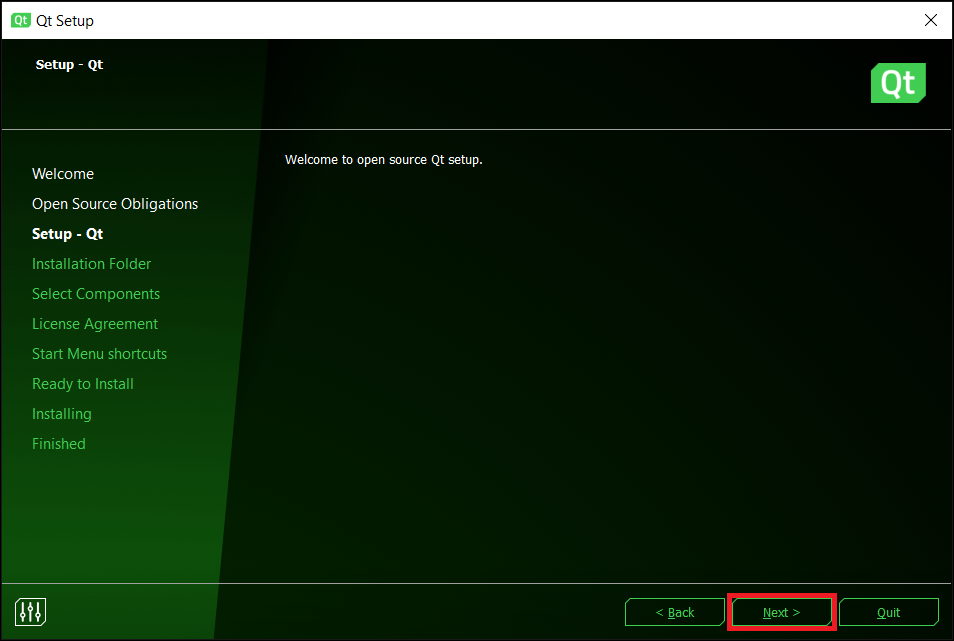
\includegraphics[width=12cm]{img/kap04_inst_set}
	\caption{\uv{Setup - Qt} časť Qt Setupu}
	\label{obr:kap4:inst_set}
\end{figure}

\item Teraz zaškrtneme jednu z možností o zasielaní štatistických údajov počas používania Qt Creatoru. Tu si môžeme zvoliť ktorúkoľvek z možností podľa osobných preferencií. Následne klikneme na tlačidlo \uv{Next} (obrázok~\ref{obr:kap4:inst_cont}).

\begin{figure}[!htb]
	\centering
	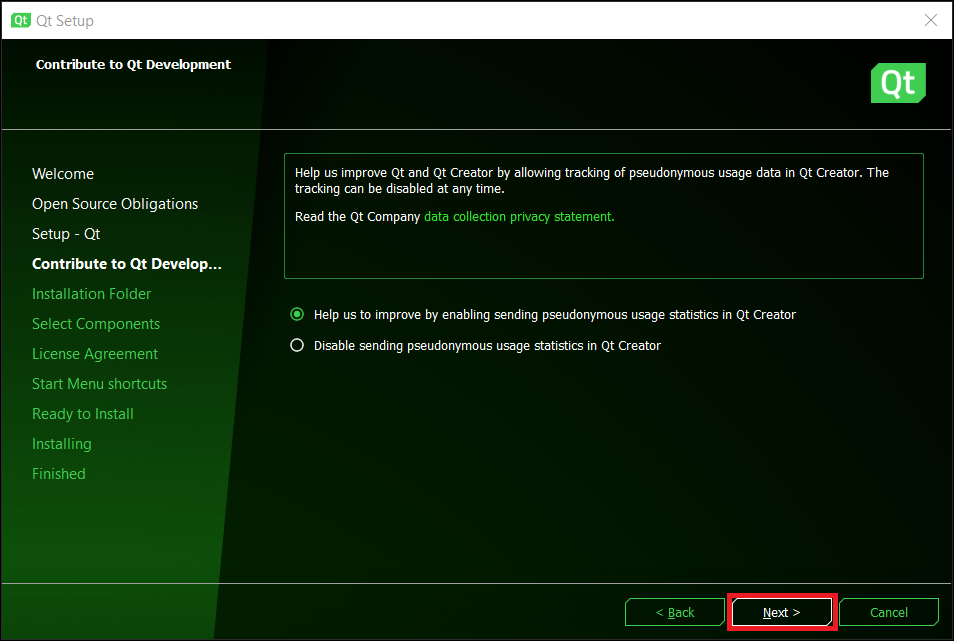
\includegraphics[width=12cm]{img/kap04_inst_cont}
	\caption{\uv{Contribute to Qt Development} časť Qt Setupu}
	\label{obr:kap4:inst_cont}
\end{figure}

\item Na tejto obrazovke (obrázok~\ref{obr:kap4:inst_int}) si zvolíme adresár do ktorého chceme Qt nainštalovať a zaklikneme možnosť \uv{Custom installation}. Následne klikneme na \uv{Next}.

\begin{figure}[!htb]
	\centering
	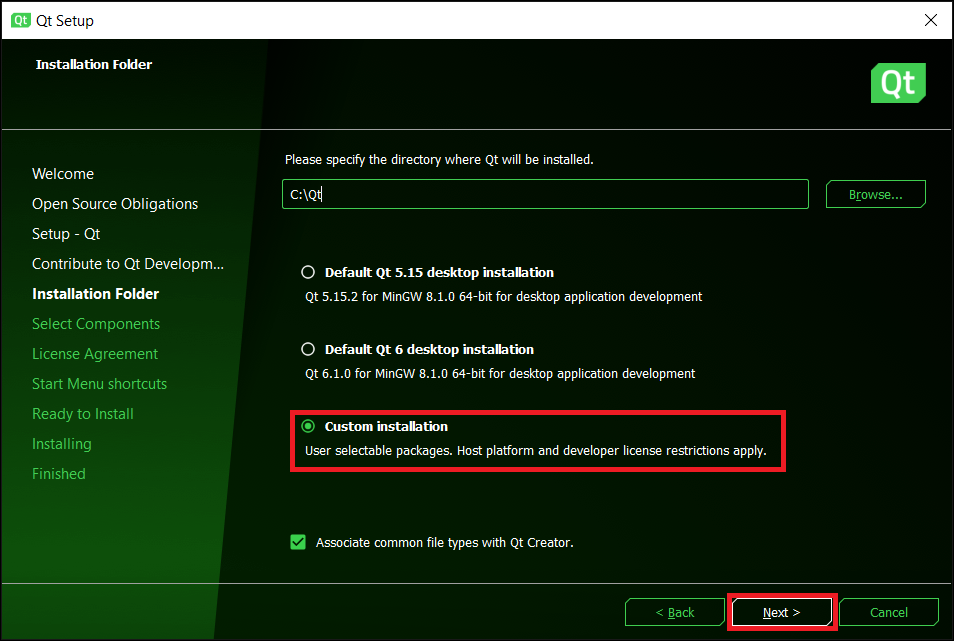
\includegraphics[width=12cm]{img/kap04_inst_int}
	\caption{\uv{Installation Folder} časť Qt Setupu}
	\label{obr:kap4:inst_int}
\end{figure}

\item Teraz si zvolíme konkrétne komponenty, ktoré sa nám nainštalujú. Komponenty, ktoré sú zaškrtnuté necháme tak a rozklikneme možnosť Qt$\leftarrow$Qt 5.15.0 a zaškrtneme možnosť \uv{MSVC 2019 64-bit} a klikneme na \uv{Next} (obrázok~\ref{obr:kap4:inst_sel}).

\begin{figure}[!htb]
	\centering
	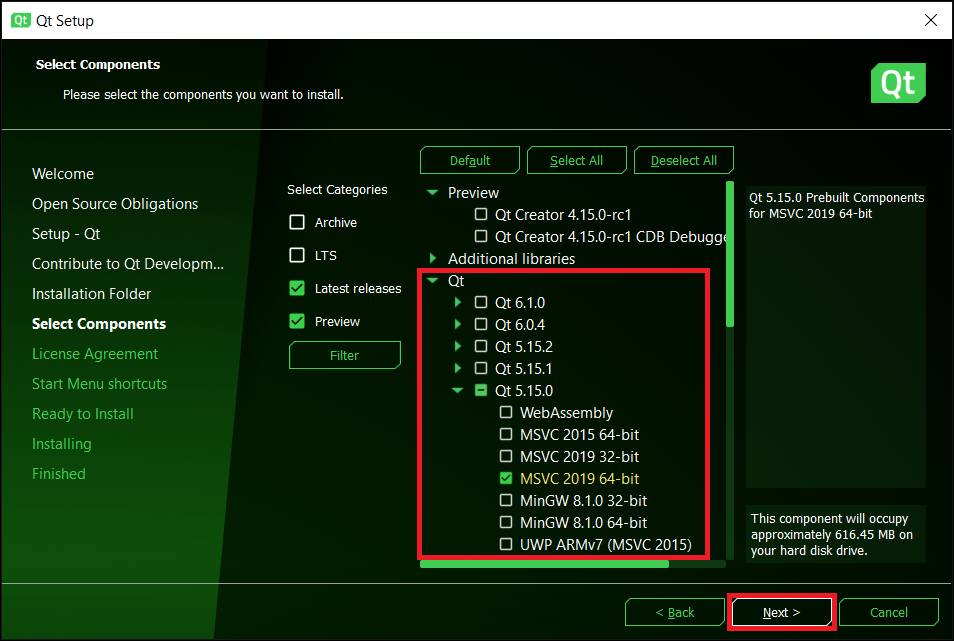
\includegraphics[width=12cm]{img/kap04_inst_sel}
	\caption{\uv{Select Components} časť Qt Setupu}
	\label{obr:kap4:inst_sel}
\end{figure}

\item Na aktuálnej obrazovke (obrázok~\ref{obr:kap4:inst_lic}) zaškrtneme možnosť, že sme si prečítali a súhlasíme s licenčnej zmluvy a klikneme na \uv{Next}.

\begin{figure}[!htb]
	\centering
	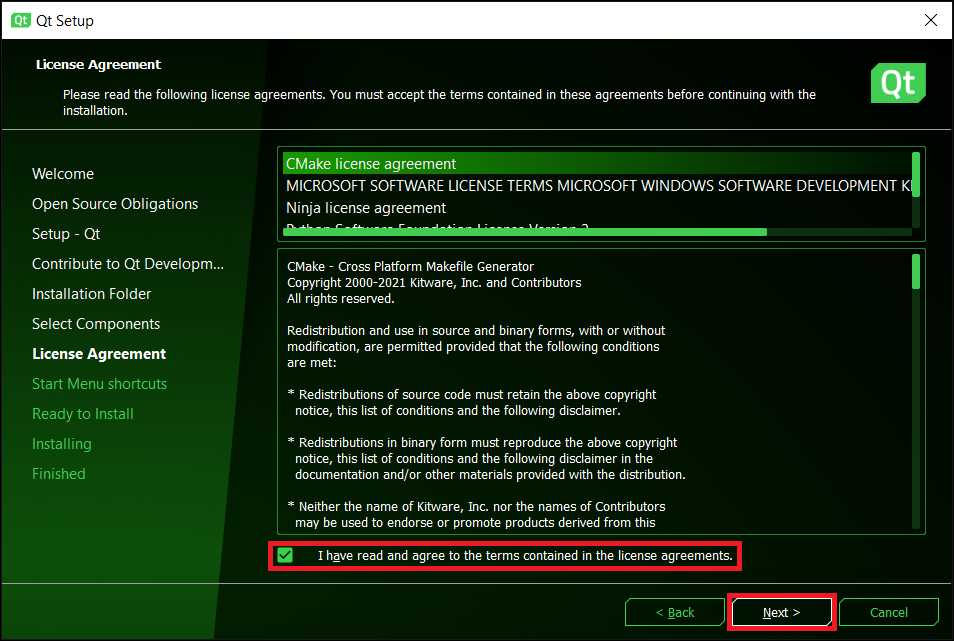
\includegraphics[width=12cm]{img/kap04_inst_lic}
	\caption{\uv{License Agreement} časť Qt Setupu}
	\label{obr:kap4:inst_lic}
\end{figure}

\item Zvolíme si start menu skratku a klikneme na \uv{Next} (obrázok~\ref{obr:kap4:inst_star}).

\begin{figure}[!htb]
	\centering
	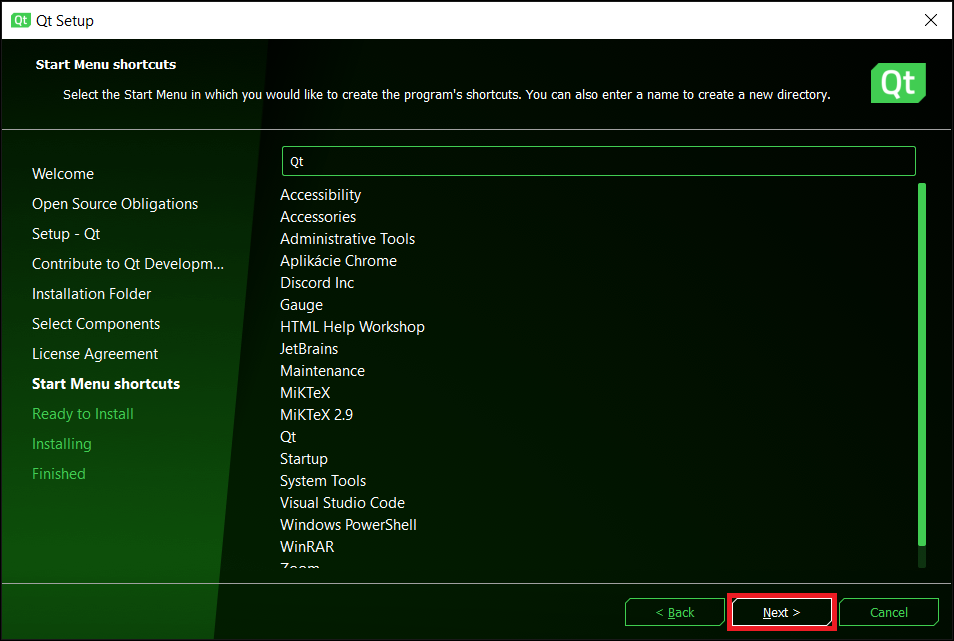
\includegraphics[width=12cm]{img/kap04_inst_star}
	\caption{\uv{Start Menu Shortcut} časť Qt Setupu}
	\label{obr:kap4:inst_star}
\end{figure}

\item Teraz už len klikneme na \uv{Install} (obrázok~\ref{obr:kap4:inst_ready}) a počkáme kým prebehne inštalácia.

\begin{figure}[!htb]
	\centering
	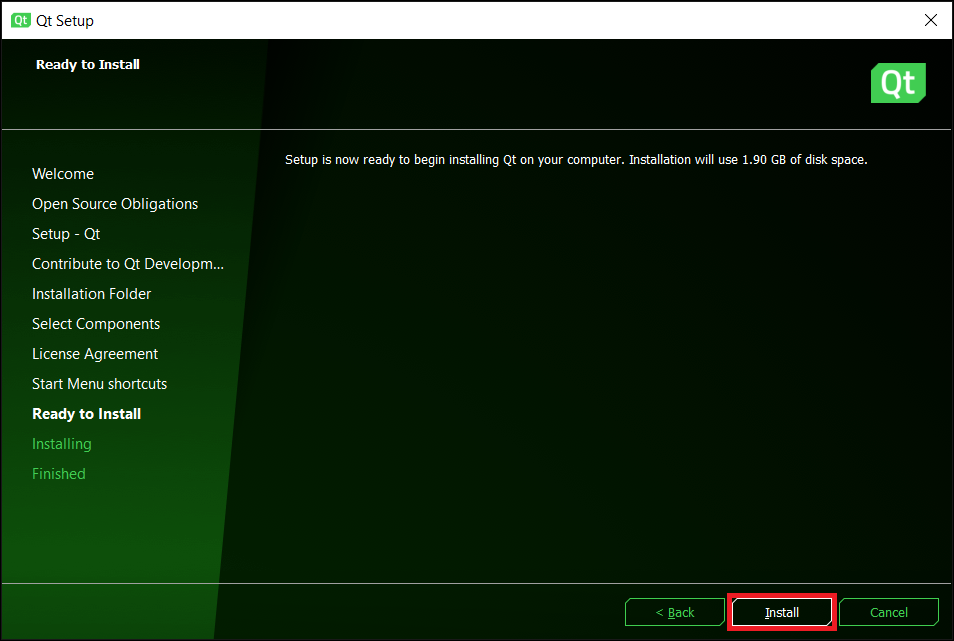
\includegraphics[width=12cm]{img/kap04_inst_ready}
	\caption{\uv{Ready to Install} časť Qt Setupu}
	\label{obr:kap4:inst_ready}
\end{figure}

\item V záverečnej obrazovke môžeme odškrtnúť možnosť \uv{Launch Qt Creator} a klikneme na tlačidlo \uv{Finish}.

\end{itemize}

\clearpage

\subsection{Visual Studio 2019 a Qt}
\label{kap4:sec:VS2019_qt}
Teraz si ešte ukážeme integrovanie Visual studia 2019 spolu s Qt. Budeme si potrebovať nainštalovať \textit{Qt VS Tools}. Podrobný postup si ukážeme v nasledujúcich krokoch:
\begin{itemize}
\label{kap4:qt_vs_integ}
\item Priamo vo Visual Studiu si cez možnosť \textit{Extensions}$\rightarrow$\textit{Manage Extensions} do online hľadania zadáme \uv{Qt} a stiahneme si rozšírenie \uv{Qt Visual Studio Tools}~\cite{qt_vs_tools}
\item\label{kap4:qt_vs_integ:krok2} Po úspešnej inštalácii si musíme ešte vybrať Qt verziu cez možnosť \textit{Extensions}$\rightarrow$\textit{Qt VS Tools}$\rightarrow$\textit{Qt Versions} (ukázané na obrázku~\ref{obr:kap4:vs_versions}).

\begin{figure}[!htb]
	\centering
	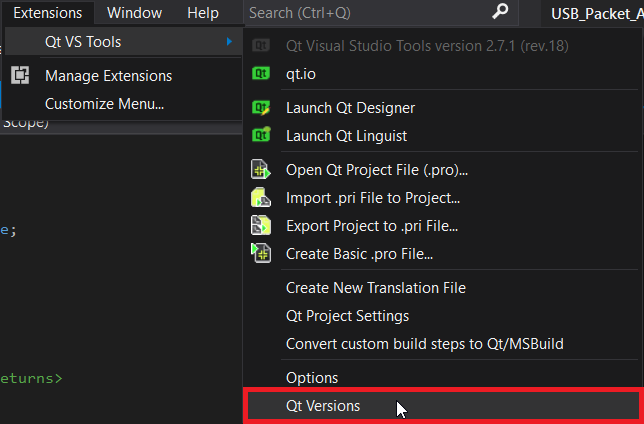
\includegraphics[width=12cm]{img/kap04_vs_versions}
	\caption{Visual Studio možnosť vybratia Qt verzie.}
	\label{obr:kap4:vs_versions}
\end{figure}

\item V dialógu sa teraz cez ikonu v stĺpčeku \uv{Path} (obrázok~\ref{obr:kap4:vs_path}) odkážeme do adresáru, kde sme nainštalovali \textit{Qt} a následne do adresáru \textit{5.15.0\/msvc2019\_64\/bin} kde máme nainštalovaný \textit{qmake.exe}.

\begin{figure}[!htb]
	\centering
	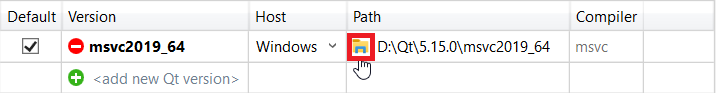
\includegraphics[width=12cm]{img/kap04_vs_path}
	\caption{Visual Studio zvolenie adresára ku \textit{qmake.exe}.}
	\label{obr:kap4:vs_path}
\end{figure}

\item Ako posledné si ešte skontrolujeme cez možnosť \textit{Project}$\rightarrow$\textit{Properties} v \textit{Configuration Properties}$\rightarrow$\textit{General} skontrolujeme, že máme nastavený \textit{C++ Language Standard} na možnosť \textit{ISO C++ 17} a \textit{Windows SDK Version} na verziu \textit{10.0.19041.0} ako na obrázku~\ref{obr:kap4:vs_prop}.

\begin{figure}[!htb]
	\centering
	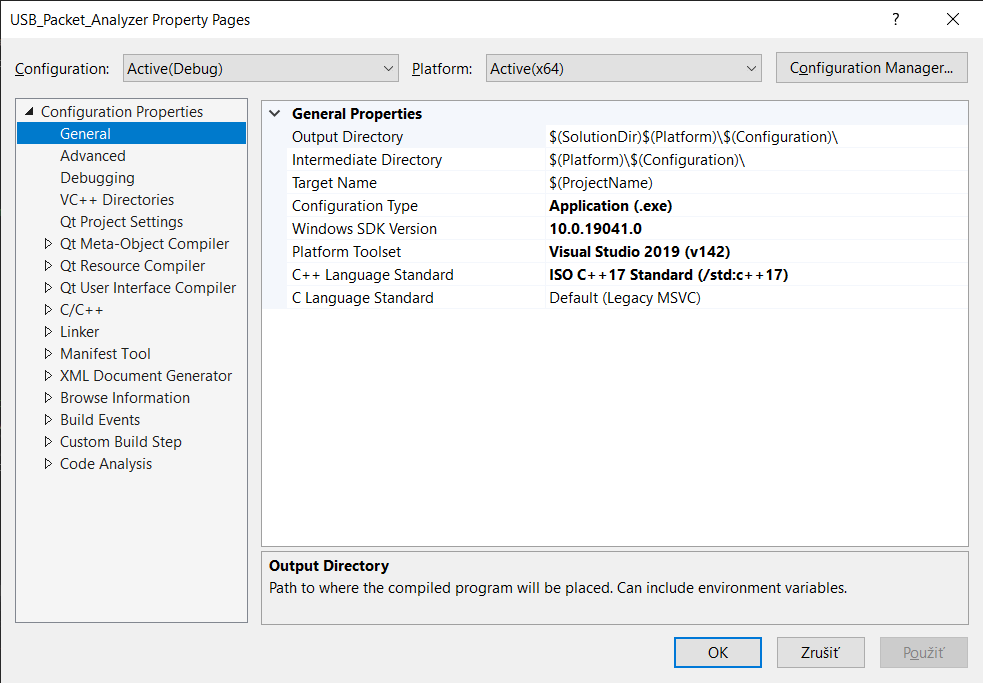
\includegraphics[width=12cm]{img/kap04_vs_prop}
	\caption{Visual Studio obecné nastavenia projektu.}
	\label{obr:kap4:vs_prop}
\end{figure}

\end{itemize}

Môže sa stať, že narazíme na bug keď nám krok~\ref{kap4:qt_vs_integ:krok2} nenastaví Qt verziu a nebudeme vedieť projekt preložiť kvôli errorom typu \uv{cannot open source file qbytearray}. V takom prípade prejdeme do možnosti \textit{Project}$\rightarrow$\textit{Properties}$\rightarrow$\textit{Qt~Project~Settings} a manuálne nastavíme \textit{Qt Installation} na \textit{msvc2019\_64} (obrázok~\ref{obr:kap4:vs_manual}).

\begin{figure}[!htb]
	\centering
	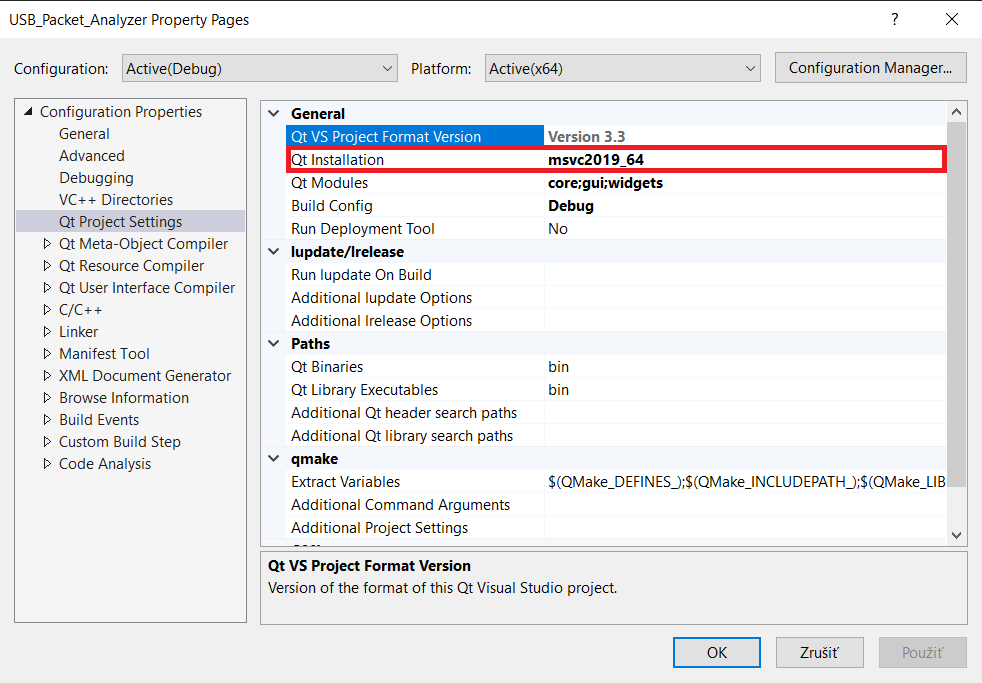
\includegraphics[width=12cm]{img/kap04_vs_manual}
	\caption{Visual Studio manuálne nastavenie Qt Installation.}
	\label{obr:kap4:vs_manual}
\end{figure}

V tomto momente by sme mali byť schopní úspešne skompilovať a spustiť náš program.

\newpage

\section{Architektúra aplikácie}

\begin{figure}[!htb]
	\centering
	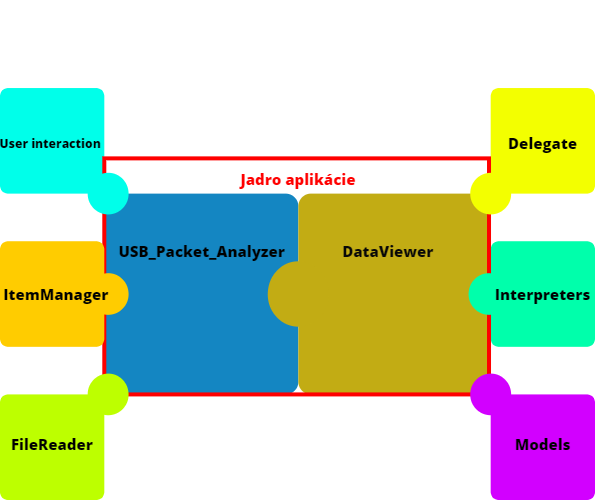
\includegraphics[width=\textwidth]{img/kap04_architektura}
	\caption{Diagram architektúry aplikácie}
	\label{obr:kap4:architek}
\end{figure}

V tejto sekcii si prejdeme celkovú stavbu aplikácie a akým spôsobom sú jednotlivé komponenty prepojené. Ako vidíme na obrázku~\ref{obr:kap4:architek}, aplikáciu môžeme rozdeliť do dvoch hlavných komponent, ktoré tvoria logické jadro programu: \texttt{USB\_Packet\_Analyzer} a \texttt{DataViewer}, na ktoré sa viažu ďalšie komponenty a dopĺňajú ich funkcionalitu. Teraz si podrobnejšie opíšeme obe hlavné komponenty spolu s komponentami, ktoré sú na nich napojené.

\subsection{USB\_Packet\_Analyzer}

USB\_Packet\_Analyzer tvorí hlavnú triedu programu, ktorá reprezentuje okno zobrazené užívateľovi hneď po zapnutí aplikácie. Naše hlavné okno pozostáva z nasledujúcich komponent:
\begin{itemize}
\item QTableWidget -- slúži na vyobrazenie základných informácií o paketoch.
\item 2 QRadioButtony -- slúžia na výber medzi analýzou fixného súboru (file capture), alebo súboru do ktorého môže sniffer počas analýzy niečo pripísať (live capture).
\item QCheckBox -- slúži na výber, či užívateľ chce farebne zvýrazniť detailnejší význam analyzovaných paketov alebo nie.
\item QLabel -- slúži na vyobrazenie názvu súboru, ktorý sa aktuálne spracováva.
\item QProgressBar -- progress bar ukazujúci stav spracovania súboru počas file capture.
\item 5 QPushButtonov -- tlačidlá, ktorých jednotlivú funkcionalitu si vysvetlíme nižšie v tejto sekcii~\ref{kap04:sec:open_button}.
\end{itemize}
Zároveň implementuje funkcie spojené s užívateľskou interakciou, od ktorej sa následne odvíja ďalšie správanie aplikácie.

\subsubsection{Užívateľská interakcia}
Ako sme už spomínali vyššie v kapitole~\ref{kap3:sec:model_view}, Qt využíva na komunikáciu medzi objektami tzv. \uv{Signals \& Slots}~\cite{signal_slot} mechanizmus, ktorý funguje ako alternatíva ku callback funkciám v iných frameworkoch. Qt widgety majú veľa preddefinovaných signálov (ku ktorým si môžeme dodefinovať ďalšie), ktoré sú emitované pri konkrétnom evente (napríklad QPushButton~\cite{qpushbutton} má signál \texttt{clicked()} ktorý je emitnutý pokiaľ je dané tlačidlo stlačené). Slot je funkcia, ktorá je zavolaná ako odpoveď na konkrétny signál. Prepojenie signálu so slotom prebieha pomocou metódy \texttt{QObject::connect(QObject* sender, signal, QObject* receiver, method)}, kde postupne definujeme inštanciu QObject spolu s jej konkrétnym signálom a následne inštanciu QObject spolu s jej metódou, ktorá sa má zavolať po emitovaní daného singálu. Qt má takisto možnosť \uv{Auto-Connect}~\cite{qt_autoconnect} pri ktorej stačí, že sa budeme držať štandardných konvencií a tým pádom nebudeme musieť manuálne prepájať jednotlivé signály a sloty pomocou \texttt{connect()} metódy. Toto využívame napríklad pri tlačidlách, konkrétne so signálom \texttt{clicked()}, kde stačí ak si vytvoríme slot pomocou nasledujúcej mennej konvencie: \texttt{void on\_\textless object name \textgreater\_clicked()}.

\begin{figure}[!htb]
	\centering
	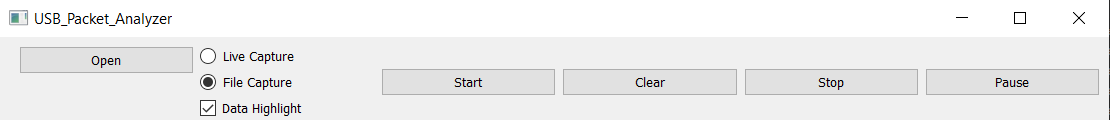
\includegraphics[width=\textwidth]{img/kap04_arch_buttons}
	\caption{Tlačidlá v aplikácii.}
	\label{obr:kap4:arch:buttons}
\end{figure}

Ako môžeme vidieť na obrázku~\ref{obr:kap4:arch:buttons}, naša aplikácia obsahuje hneď niekoľko tlačidieľ s odlišnou funkcionalitou o ktorú sa starajú už jednotlivé sloty, ktoré si teraz postupne opíšeme.

\paragraph{Open tlačidlo}
\label{kap04:sec:open_button}

slúži na vybratie si súboru na analýzu. To funguje na základe triedy QFileDialog~\cite{qfiledialog}, ktorá slúži na prechádzanie file systému. Užívateľovi sa zobrazí nový dialóg s intuitívnym ovládaním na ktoré je bežný užívateľ zvyknutý. Zároveň slúži na resetovanie progress baru a nastavenie labelu, ktorý zobrazuje aktuálne zvolený súbor.

\paragraph{Start tlačidlo}

ako už napovedá jeho samotný názov, slúži na začatie analýzy. V tejto chvíli sa začne spracovávať súbor, ktorý si užívateľ zvolil pomocou predcházajúceho tlačidla Open~\ref{kap04:sec:open_button}. Spracovanie je následne vyobrazené pomocou QTableWidgetu, ktorým ako sme už riešili v kapitole~\ref{kap03:sec:zobr_zakl} vyobrazujeme základné informácie o jednotlivých paketoch. O cekové spracovanie súboru a jeho vyobrazenie tak ako aj o iné veci, sa stará trieda \textit{ItemManager}, o ktorej si povieme viac neskôr v sekcii (ODKAZ).

\paragraph{Clear tlačidlo}

zastáva funkciu vyčistenia plochy QTableWidgetu na ktorej sú vyobrazné základné informácie o paketoch. Takisto resetne progress bar, ktorým reprezentujeme v akom stave sa nachádzame z hľadiska spracovania daného súboru.

\paragraph{Stop tlačidlo}

spôsobí to, že sa úplne zastaví spracovávanie súboru. Využívané je pri analýze paketov v reálnom čase, čím stopne pridávanie nových paketov do QTableWidgetu. Akékoľvek ďalšie spracovávanie súborov už nie je umožnené. Ak by sme chceli analýzu len pozastaviť, tak v takom prípade použijeme tlačidlo Pause~\ref{kap04:sec:pause_button}.

\paragraph{Pause tlačidlo}
\label{kap04:sec:pause_button}

ako už bolo naznačené vyššie, slúži na pozastavenie analýzy. To znamená, že nové pakety nie sú pridávané do QTableWidgetu. Obnovenie analýzy je možné opätovným stlačením tlačidla (teraz už s nápisom \uv{Continue}), čím bude obnovené pridávanie nových paketov.

Z užívateľskej interakcie máme k dispozícii ešte jednu, o ktorej sme viac hovorili v kapitole~\ref{kap03:sec:zobr_zakl}, kde sme sa pre splnenie požiadavky na vyobrazenie detailnejších informácií o pakete na základe užívateľskej interakcie rozhodli pre dvojklik na položku reprezentujúcu daný paket.

\paragraph{\texttt{on\_tableWidget\_itemDoubleclicked(QTableWidget* item)}}

je slot, ktorý sa volá po dvojkliku na konkrétny item v QTableWidget (pointer na daný item je poslaný ako parameter). V tejto metóde vytvoríme novú inštanciu triedy DataViewer s odpovedajúcimi parametrami a vyobrazíme jej dialógové okno, ktoré zobrazí detailnejšie informácie o danom pakete.

\subsubsection{ItemManager}
Interakciu užívateľa so systémom sme si už vysvetlili, poďme sa teraz pozrieť na samotné spracovávanie súborov.

%Budeme si potrebovať nainštalovať Qt pre Windows. podla videa, verzia 5.15.0 len msvc 2019 64bit. inak ostatne default. zatial som este nainstaloval QT VS extension. teraz idem updatenut SDK na verziu 10.0.19041.0 -- to vymazalo errory typu ''cannot open source file cctype'' , teraz mi este ostali ''cannot open source file qbytearray'' a podobne spojene cisto s qt : pravdepodobne bug. musel som ist manualne do Project->properties->Qt Project SEttings a nastavit Qt installation na verziu 5.15.0_msvc2019_64. A UZ TO BEZIIII :)



























\newpage
\section{Architekrúra aplikácie}
\section{Jadro aplikácie}
\subsection{USB\_Packet\_Analyzer}
riadi celkovy beh programu, reaguje na input od uzivatela
\subsection{Item Manager}
spracovanie samostatneho packetu a ulozenie dat o nom
\subsection{DataViewer}
trieda ktora ma na starosti vyskakovacie okno po dvojkliku a item a nasledne reaguje na input od uzivatela v okne
\subsection{TreeItem}
reprezentuje jednotlive nody v stromovej strukture ktora sa potom vyuziva na zobrazenie dat v QTreeView
\section{Modely}
\subsection{AdditionaldataModel}
model na spravovanie zvysnych dat(data ktore nie su sucastou hlavicky packetu)
\subsection{ColorMapModel}
vyobrazenie pomocnej mapy na lepsie sa zorientovanie v zvyraznemom hexdumpe
\subsection{DataViewerModel}
model na hexdump - prenasa hex/printable a zaroven o co vlastne ide(konkretny descriptor, interrupt data, ...)
\subsection{TreeItemBaseModel}
model na QTreeView ktorz vyuziva TreeItem
\subsection{USBPcapHeaderModel}
model na QTreeView ale specialne pre USBPcap hlavicku packetu
\section{Interpretery}
\subsection{BaseInterpreter}
abstractna trieda od ktorej dedia vsetkz interpretery
\subsection{Interpreter factory}
facory trieda na pridelenie konkretneho interpreteru za runtimu kvoli jednoduchosti na lepsie rozsirenie programu do buducnosti
\subsection{Interpretery descriptorov}
Config,Device,Setup,String,...
\subsection{Interrupt transfer interpretery}
obecne interrupt transfer interpreter - sluzi skor ako factory na rozne doteraz implementovane HID zariadenia
\subsubsection{Joystick interpreter}
\subsubsection{Mouse interpreter}
\subsubsection{Keyboard interpreter}
\section{Delegáti}
\subsubsection{DataViewerDelegate}
Qt delegat - stara sa o highlight hexdumpu
\section{HID}
\subsection{HIDDevices}
staticka trieda, drzi vsetky rozpoznane HID zariadenia a obsahuje funkcie specificke nich - parsovanie HID Report descriptoru
\section{Práca so súbormi}
\subsection{FileReader}
praca zo suborom a predavanie precitanych dat, offline/online capture, QFile vs std::istream
\section{Globálne dáta}
\subsection{ConstDataHolder}
staticka trieda na drzanie si konstant ktore su potrebne napriec celym programom. Mapovanie z enumu do jeho stringovej reprezentacie
\subsection{PacketExternStructs}
obsahuje definiciu vsetkych dolezitych USBPcap structov, pcap structov, enumov a vsetkych structov ktore pouzivam v aplikacii











